\documentclass{article}
\usepackage[utf8]{inputenc}
\usepackage[margin=3.0cm]{geometry}
\usepackage{minted}
\usepackage{amssymb}
\usepackage{amsthm}
\usepackage{amsmath}
\usepackage{graphicx}
\usepackage{bbm}
\usepackage{subcaption}
\pagestyle{empty}
\usepackage[table]{xcolor}
\newcommand{\wo}{\mathbbm{w}}

\pdfinfo{
/Title (report2)
/Author (Felipe Salvatore)}
\setcounter{secnumdepth}{0}  


\title{Report: assigment 2}
\author{Felipe Salvatore\\
\texttt{felipessalvador@googlemail.com}}
\begin{document}
\maketitle
\section{1}
\textbf{1a)} 
\begin{minted}{python}
def softmax(x):
    # ## YOUR CODE HERE
    all_constants = - tf.reduce_max(x, axis=1)
    x = x + tf.expand_dims(all_constants, 1)
    x = tf.exp(x)
    all_sums = tf.reduce_sum(x, 1)
    all_sums = tf.pow(all_sums, -1)
    out = x*tf.expand_dims(all_sums, 1)
    # ## END YOUR CODE
    return out
\end{minted}


\textbf{1b)}
\begin{minted}{python}
def cross_entropy_loss(y, yhat):
    # ## YOUR CODE HERE
    y = tf.cast(y, tf.float32)
    yhat = tf.log(yhat)
    out = - tf.reduce_sum(y*yhat)
    out = tf.reshape(out, (1,))
    # ## END YOUR CODE
    return out
\end{minted}

\textbf{1c)} The placeholders variables are like their name suggest a placeholder for a tensor. We use it to form a computational graph before the training. In the training stage we use the dictionary feed\_dict to 'load' the placeholders variables with real tensors.

\begin{minted}{python}
    def add_placeholders(self):
        # ## YOUR CODE HERE
        self.input_placeholder = tf.placeholder(tf.float32,
                                                shape=[self.config.batch_size,
                                                       self.config.n_features],
                                                name="input_placeholder")
        self.labels_placeholder = tf.placeholder(tf.int32,
                                                 shape=[self.config.batch_size,
                                                        self.config.n_classes],
                                                 name="labels_placeholder")
        # ## END YOUR CODE

    def create_feed_dict(self, input_batch, label_batch):
        # ## YOUR CODE HERE
        feed_dict = {self.input_placeholder: input_batch,
                     self.labels_placeholder: label_batch}
        # ## END YOUR CODE
        return feed_dict
\end{minted}

\textbf{1d)}
\begin{minted}{python}
    def add_model(self, input_data):
        Wshape = [self.config.n_features, self.config.n_classes]
        bshape = [self.config.batch_size, self.config.n_classes]
        Winit = tf.zeros(Wshape)
        binit = tf.zeros(bshape)

        with tf.variable_scope("linear-model"):
            W = tf.get_variable("weights", dtype='float32', initializer=Winit)
            b = tf.get_variable("bias", dtype='float32', initializer=binit)
            out = softmax(tf.matmul(input_data, W) + b)
        # ## END YOUR CODE
        return out

    def add_loss_op(self, pred):
        # ## YOUR CODE HERE
        loss = cross_entropy_loss(self.labels_placeholder,
                                  pred)
        # ## END YOUR CODE
        return loss
\end{minted}


\textbf{1e)}
\begin{minted}{python}
    def add_training_op(self, loss):
        # ## YOUR CODE HERE
        optimizer = tf.train.GradientDescentOptimizer(self.config.lr)
        train_op = optimizer.minimize(loss)

        # ## END YOUR CODE
        return train_op
\end{minted}
All the basic operations in TensorFlow have attached
gradient operations. And so with the use of backpropagation TensorFlow computes the gradients for all variables in the computation graph.

\section{2}
We shall first understand \textbf{the Named Entity Recognition (NER) window model}. Suppose we have a corpus with a vocabulary $V =[\wo_{1}, \dots, \wo_{|V|}]$ (we are assuming that every word $\wo$ correspond to an index $i \in \{1, \dots, |V|\}$), a number $C$ of name entity categories (null-class,Person, Location, etc.) and a matrix $L \in \mathbb{R}^{|V|,d}$ where each row $i$ correspond to the word embedding of size $d$ of the word $\wo_{i}$. Now we can choose the parameters $m$ and $H$ to be the size window and the size of the hidden layer, respectively. Let $n = (2m+1)d$, $W \in \mathbb{R}^{n,H}$, $b_{1} \in \mathbb{R}^{H}$, $U \in \mathbb{R}^{H,C}$ and $b^{2} \in \mathbb{R}^{C}$. We assume that the training dataset is compose by training samples of the form $([\wo_{t-m}, \dots, \wo_{t}, \dots, \wo_{t+m}],c)$ where $c \in \{1, \dots, C\}$ ($1$ represent the null-class) -- this sample tell us that the word $ \wo_{t}$ is a name entity of type $c$. Let $y$ be the one-vector representation of $c$ (i.e., $y \in \mathbb{R}^{C}$ such that $y_{i} =1$ iff $i=c$), and let $x_{t-m}, \dots, x_{t}, \dots, x_{t+m}\in \mathbb{R}^{|V|}$ be the one-vector representation of $\wo_{t-m}, \dots, \wo_{t}, \dots, \wo_{t+m}$, respectively. The model is composed by the following equations:
\begin{equation}\label{eq:0}
x^{(t)} = concat([x_{t-m}L, \dots, x_{t}L, \dots, x_{t+m}L])
\end{equation}
\begin{equation}\label{eq:1}
z = x^{(t)}W + b_{1}
\end{equation}
 \begin{equation}\label{eq:2}
h = tanh(z)
\end{equation}
\begin{equation}\label{eq:3}
\hat{y} = softmax(hU + b_{2})
\end{equation}
\begin{equation}\label{eq:4}
J(W,b_{1},U,b_{2}) = CE(y,\hat{y}) = -\sum_{s=1}^{C} y_s  \log(\hat{y}_s)
\end{equation}

where $concat$ is the operation of concatenate function and $tanh$ is the hyperbolic tangent function ,i.e.,  $tanh(z) = \frac{e^{z} - e^{-z}}{e^{z} + e^{-z}}$, we can define this function using the sigmoid function, $tanh(z) = 2sigmoid(2z)-1$. Figure \ref{ner} helps us to visualize the model.

For our particular implementation, let $C=5$ $d=50$, $m=1$, $H=100$ (hence $n=150$) and let $J(\theta)$ be an abbreviation of $J(W,b_{1},U,b_{2})$. Thus, for every training sample the loss function is
\begin{equation}\label{eq:5}
J(\theta) = CE(y,\hat{y}) = -\sum_{s=1}^{5} y_s  \log(\hat{y}_s)
\end{equation}


\begin{figure}
\begin{center}
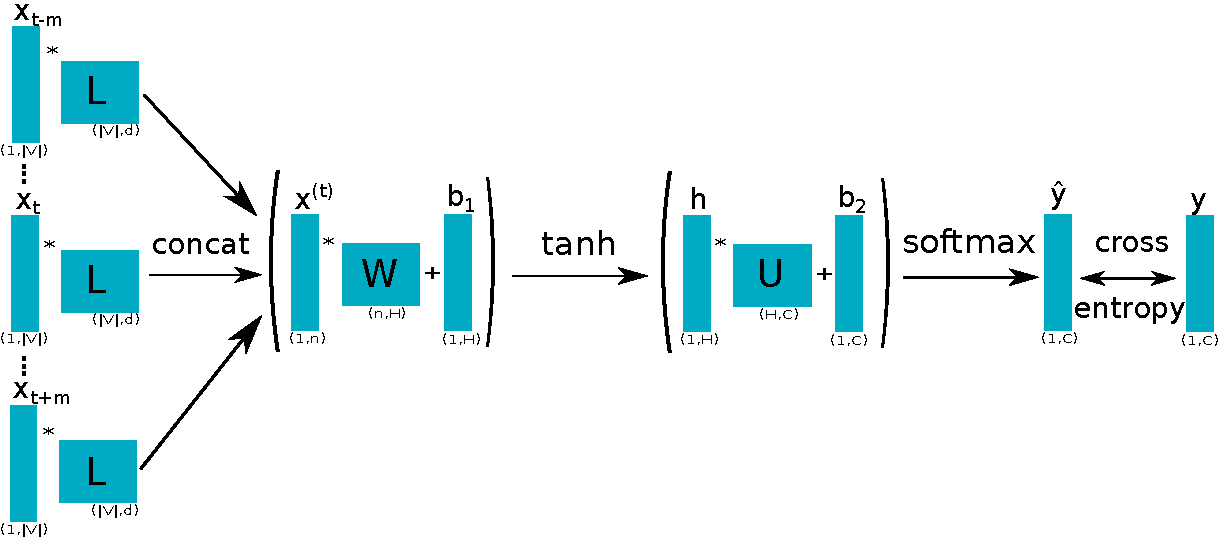
\includegraphics[scale=0.85]{ner.pdf}
\end{center}
\caption{NER window model}
\label{ner}
\end{figure}
\textbf{2a)} Since $tanh(z) = 2\sigma(2z) -1 $ we have that, 
\begin{align*}
tanh^{\prime}(z) & = 2\sigma^{\prime}(2z)2 \\
& =4\sigma^{\prime}(2z) \\
& = 4(\sigma(2z)(1 - \sigma(2z))) \\
& = 4\sigma(2z)(4 - 4\sigma(2z))\\
& =  2(tanh(z)+1)(4 - 2(tanh(z)+1))\\
& = 2((tanh(z)+1)(2 - (tanh(z)+1)))\; .
\end{align*}
Let $\delta^{(3)} = \hat{y} - y \in \mathbb{R}^{5}$ be the outermost error vector, hence

\begin{equation}\label{eq:6}
\frac{\partial J}{\partial  U} = {h \delta^{(3)}}^{T}
\end{equation}

\begin{equation}\label{eq:7}
\frac{\partial J}{\partial  b_{2}} =  \delta^{(3)}
\end{equation}

\begin{equation}\label{eq:8}
\delta^{(2)} = (\delta^{(3)} {(U)}^{T}) \circ {tanh^{\prime}} (z)
\end{equation}

\begin{equation}\label{eq:9}
\frac{\partial J}{\partial  W} = {x^{(t)} \delta^{(2)}}^{T}
\end{equation}

\begin{equation}\label{eq:10}
\frac{\partial J}{\partial  b_{1}} =  \delta^{(2)}
\end{equation}

First let us define $\frac{\partial J}{\partial  L_{i}}$ for the general case. Using the fact that $\frac{\partial J}{\partial  x^{(t)}}= \delta^{(2)} {(W)}^{T}$ we will define the auxiliary vectors  $v_{1}, \dots, v_{2m+1} \in \mathbb{R}^{d}$ such that for $j \in \{ 1, \dots, 2m+1\}$ 
\begin{equation}\label{eq:11}
v_{j} =  \frac{\partial J}{\partial  x^{(t)}}[(j-1)d +1: jd]
\end{equation}

Let $e$ be the enumeration function of the list $[t-m, \dots, t, \dots, t+m]$, so for $i \in \{ t-m, \dots, t, \dots, t+m \}$

\begin{equation}\label{eq:12}
\frac{\partial J}{\partial  L_{i}} =  v_{e(i)}
\end{equation}

And for $i \notin \{ t-m, \dots, t, \dots, t+m \}$ $\frac{\partial J}{\partial  L_{i}} =0$. Now for the specific case where $m=1$, 

\begin{equation}\label{eq:13}
\frac{\partial J}{\partial  L_{t-1}} =  \frac{\partial J}{\partial  x^{(t)}}[1: d]
\end{equation}
\begin{equation}\label{eq:14}
\frac{\partial J}{\partial  L_{t}} =  \frac{\partial J}{\partial  x^{(t)}}[d+1: 2d]
\end{equation}
\begin{equation}\label{eq:15}
\frac{\partial J}{\partial  L_{t+1}} =  \frac{\partial J}{\partial  x^{(t)}}[2d+1: 3d]
\end{equation}

And for $i \notin \{ t-m, \dots, t, \dots, t+m \}$ $\frac{\partial J}{\partial  L_{i}} =0$.

\textbf{2b)} To add L2 regularization to our model, we can add the following function:
\begin{equation}\label{eq:16}
J_{reg}(\theta) = \frac{\lambda}{2}[\sum_{i=1}^{n}\sum_{j=1}^{H}(W_{i,j})^{2}) + \sum_{i^{\prime}=1}^{H}\sum_{j^{\prime}=1}^{C}(U_{i^{\prime},j^{\prime}})^{2})]
\end{equation}

where $\lambda \in \mathbb{R}$ is the regularization parameter. Hence,

\begin{equation}\label{eq:17}
J_{full}(\theta) =J(\theta) + J_{reg}(\theta)
\end{equation}

The only grandients that change are in respect to $U$ and $W$. Let $\delta^{(3)}$ and $\delta^{(2)}$ be as before; then,

\begin{equation}\label{eq:18}
\frac{\partial J_{full}}{\partial  U} = {h \delta^{(3)}}^{T} + \lambda U 
\end{equation}

\begin{equation}\label{eq:19}
\frac{\partial J_{full}}{\partial  b_{2}} =  \frac{\partial J}{\partial  b_{2}}
\end{equation}

\begin{equation}\label{eq:20}
\frac{\partial J_{full}}{\partial  W} = {x^{(t)} \delta^{(2)}}^{T} + \lambda W 
\end{equation}

\begin{equation}\label{eq:21}
\frac{\partial J_{full}}{\partial  b_{1}} =  \frac{\partial J}{\partial  b_{1}} 
\end{equation}
And for $i \in \{1, \dots, |V|\}$
\begin{equation}\label{eq:22}
\frac{\partial J_{full}}{\partial  L_{i}} =  \frac{\partial J}{\partial  L_{i}} 
\end{equation}

\textbf{2c)}
\begin{minted}{python}
def xavier_weight_init():
    
    def _xavier_initializer(shape, **kwargs):
        
        # ## YOUR CODE HERE
        epsilon = np.sqrt(6.)/np.sqrt(np.sum(shape))
        out = tf.random_uniform(shape,
                                minval=-epsilon,
                                maxval=epsilon,
                                dtype=tf.float32,
                                name='weights')
        # ## END YOUR CODE
        return out
    return _xavier_initializer

\end{minted}

\textbf{2d)}

\begin{minted}{python}
  def add_placeholders(self):
        # ## YOUR CODE HERE
        self.input_placeholder = tf.placeholder(tf.int32,
                                                shape=[None,
                                                       self.config.window_size],
                                                name="input_placeholder")
        self.labels_placeholder = tf.placeholder(tf.float32,
                                                 shape=[None,
                                                        self.config.label_size],
                                                 name="labels_placeholder")
        self.dropout_placeholder = tf.placeholder(tf.float32,
                                                  shape=[],
                                                  name="dropout_value")
        # ## END YOUR CODE

    def create_feed_dict(self, input_batch, dropout, label_batch=None):
        
        # ## YOUR CODE HERE
        if label_batch is None:
            feed_dict = {self.input_placeholder: input_batch,
                         self.dropout_placeholder: dropout}
        else:
            feed_dict = {self.input_placeholder: input_batch,
                         self.labels_placeholder: label_batch,
                         self.dropout_placeholder: dropout}
        # ## END YOUR CODE
        return feed_dict

    def add_embedding(self):
        with tf.device('/cpu:0'):
            # ## YOUR CODE HERE
            Linit = tf.constant_initializer(self.wv)
            L = tf.get_variable("L",
                                shape=[len(self.wv), self.config.embed_size],
                                dtype='float32',
                                initializer=Linit)
            window = tf.nn.embedding_lookup(L, self.input_placeholder)
            window = tf.reshape(window,
                                (-1,
                                 self.config.window_size*self.config.embed_size))
        # ## END YOUR CODE
        return window

def add_model(self, window):
     
        # ## YOUR CODE HERE
        # shapes
        Wshape = (self.config.window_size*self.config.embed_size,
                  self.config.hidden_size)
        b1shape = (1, self.config.hidden_size)
        Ushape = (self.config.hidden_size, self.config.label_size)
        b2shape = (1, self.config.label_size)

        # initializers
        xavier_initializer = xavier_weight_init()
        Winit = xavier_initializer(Wshape)
        b1init = xavier_initializer(b1shape)
        Uinit = xavier_initializer(Ushape)
        b2init = xavier_initializer(b2shape)

        with tf.variable_scope("Layer"):
            self.W = tf.get_variable("weights",
                                     dtype='float32',
                                     initializer=Winit)
            self.b1 = tf.get_variable("bias",
                                      dtype='float32',
                                      initializer=b1init)
            linear_op = tf.matmul(window, self.W) + self.b1
            first_output = tf.nn.dropout(tf.tanh(linear_op),
                                         self.config.dropout,
                                         name="output")
            tf.add_to_collection("reg", tf.reduce_sum(tf.pow(self.W, 2)))
        with tf.variable_scope("Softmax"):
            self.U = tf.get_variable("weights",
                                     dtype='float32',
                                     initializer=Uinit)
            self.b2 = tf.get_variable("bias",
                                      dtype='float32',
                                      initializer=b2init)
            output = tf.nn.dropout(tf.matmul(first_output, self.U) + self.b2,
                                   self.config.dropout,
                                   name="output")
            tf.add_to_collection("reg", tf.reduce_sum(tf.pow(self.U, 2)))
        # END YOUR CODE
        return output
        
  def add_loss_op(self, y):
            # ## YOUR CODE HERE
        pred = self.labels_placeholder
        cross_entropy = tf.reduce_mean(tf.nn.softmax_cross_entropy_with_logits(y, pred))
        regularization = self.config.l2*0.5*sum(tf.get_collection("reg"))
        loss = cross_entropy + regularization
        # ## END YOUR CODE
        return loss
        
  def add_training_op(self, loss):
     
        # ## YOUR CODE HERE
        optimizer = tf.train.AdamOptimizer(self.config.lr)
        train_op = optimizer.minimize(loss)
        # ## END YOUR CODE
        return train_op
\end{minted}

After some experiments (some related plots can be seen in Figure \ref{NER_e}) we choose the following hyper parameters: $ batch\_size=84, dropout=0.991323729933, lr=0.00365884577219, l2=1.7095245617e-05$. This choice yields val\_loss = $0.156871527433$.

\begin{figure}[H] 
  \begin{subfigure}[b]{0.5\linewidth}
    \centering
    \includegraphics[width=1.05\linewidth]{NER_batch_loss.png} 
    \caption{Validation loss vs batch size} 
    \label{ner_batch} 
    \vspace{4ex}
  \end{subfigure}%% 
  \begin{subfigure}[b]{0.5\linewidth}
    \centering
    \includegraphics[width=1.05\linewidth]{NER_dropout.png} 
    \caption{Validation loss vs dropout} 
    \label{ner_dropout} 
    \vspace{4ex}
  \end{subfigure} 
  \begin{subfigure}[b]{0.5\linewidth}
    \centering
    \includegraphics[width=1.05\linewidth]{NER_lr.png} 
    \caption{Validation loss vs learning rate} 
    \label{ner_lr} 
  \end{subfigure}%%
  \begin{subfigure}[b]{0.5\linewidth}
    \centering
    \includegraphics[width=1.05\linewidth]{NER_reg.png} 
    \caption{Validation loss vs regularization} 
    \label{ner_reg} 
  \end{subfigure} 
  \caption{Experiments with the NER window model}
  \label{NER_e} 
\end{figure}

\section{3} We will use a \textbf{recurrent neural network (RNN)} to build a language model. Given words $x_{1}, \dots ,x_{n-1}$ a language model predicts the following word $x_{n}$ by modeling:
\[
P(x_{n} = v_{j} | x_{1}, \dots ,x_{n-1})
\]

where $v_{j}$ is a word in the vocabulary. The model can be described as $n-1$ feed-forward neural networks, say $NN^{(1)}, \dots,NN^{(n-1)} $ such that each $NN^{(t)}$ uses an vector from $NN^{(t-1)}$ to perform the computation on its hidden layer. Since the model is the same, we can describe each $NN^{(t)}$ as a time step. Figure \ref{RNN_re} introduces the main idea:     

\begin{figure}[H] 
\begin{center}
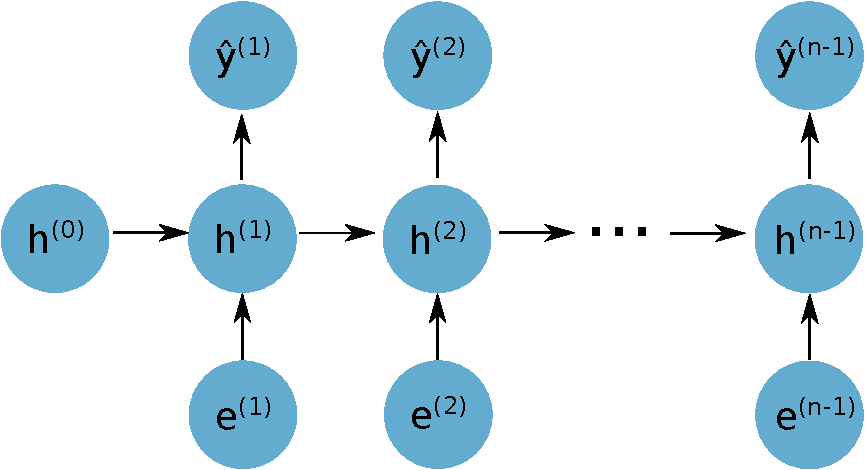
\includegraphics[scale=0.85]{RNN_ball.pdf}
\end{center}
\caption{A RNN representation}
\label{RNN_re}
\end{figure}

Since $h^{(n-1)}$ is a function of $h^{(0)},h^{(1)}, \dots, h^{(n-2)}$ we can interpret that at the time step $n-1$ the model $NN^{(n-1)}$ has the "history" of the words $x_1, x_2, \dots, x_{(n-2)}$.

To be more precise, suppose we have a corpus with a vocabulary $V$ of size $|V|$ and a matrix $L \in \mathbb{R}^{|V|,d}$ where each row $i$ correspond to the word embedding of size $d$ of the word $x_{i}$. Let $D_{h}$ be the size of the hidden layer. We use $x^{(i)} \in \mathbb{R}^{|V|}$ to be the one hot representation of $x_{i}$. We also define the following parameters: $H \in \mathbb{R}^{D_{h},D_{h}}$ is the hidden transformation matrix, $I \in \mathbb{R}^{d,D_{h}}$ is the input word representation matrix, $U \in \mathbb{R}^{D_{h},|V|}$ is the output word representation matrix, $h^{(0)} \in \mathbb{R}^{D_{h}}$ is the initialization vector for the hidden layer, and $b_{1} \in \mathbb{R}^{D_{h}}$ and $b_{2} \in \mathbb{R}^{|V|}$  are the biases. Let $x_{1}, \dots,x_{n-1}$ be a sequence of words, the target word (the one that we are trying to predict) is $x_{n}$, so for $t= 1, \dots, n-1$ the model is defined by the following equations:

\begin{equation}\label{eq:23}
e^{(t)} = x^{(t)}L
\end{equation}
 \begin{equation}\label{eq:24}
h^{(t)} = \sigma(h^{(t-1)}H + e^{(t)} I + b_{1})
\end{equation}
\begin{equation}\label{eq:25}
\hat{y}^{(t)} = softmax(h^{(t)}U + b_{2})
\end{equation}

The output vector $\hat{y}^{(t)} \in \mathbb{R}^{|V|}$ is a probability over the vocabulary, 
\begin{equation}\label{eq:26}
\hat{y}^{(t)}_{j} = P(x_{t+1} = v_{j} | x_{t}, \dots,x_{1})
\end{equation}
Let $y^{(t)} \in \mathbb{R}^{|V|}$ be the one hot representation of $x_{t+1}$, then the point-wise loss is
\begin{equation}\label{eq:27}
J(\theta)^{(t)} = CE(y^{(t)},\hat{y}^{(t)})
\end{equation}

In order to evaluate the model performance we need to compute the loss for the whole dataset. Suppose we have a dataset as a collection of $N$ words sequences, say $(x_{1,1}, \dots,x_{1,n_{1}}),\dots, (x_{N,1}, \dots,x_{1,n_{N}})$ (and let $m = \sum_{i=1}^{N}n_{i}$). For each $i=1, \dots, n_{i}$ we calculate: 
\begin{equation}\label{eq:28}
J^{(i)} = \sum_{k=1}^{(n_{i} -1)}CE(y^{(i,k)},\hat{y}^{((i,k))})
\end{equation}
where $y^{(i,s)}$ is the one hot representation of $x_{i,s+1}$. It should be noted that for each $i$ we compute $h_{0},h_{1}, \dots,h_{n_{i}}$. Since it does not make sense to use this for the next dataset entry, I think that we set $h_{0}$ with random numbers again and delete $h_{1}, \dots,h_{n_{i}}$. Hence the cross-entropy error over the dataset is:
\begin{equation}\label{eq:29}
J = -\frac{1}{m}\sum_{i=1}^{N}J^{(i)}
\end{equation}

The dataset can be a corpus with $T$ words, say $x_{1},x_{2}, \dots,x_{T}$. As before for $t = 1 ,\dots, T-1$ $y^{(t)}$ is the one hot representation of $x_{t+1}$. So the cross-entropy error over a corpus of size T is

\begin{equation}\label{eq:30}
J = -\frac{1}{T}\sum_{t=1}^{T}CE(y^{(t)},\hat{y}^{((t))})
\end{equation}

\textbf{3a)} First, let $j^{*} \in \{1, \dots, |V|\}$ be the hot index from $y^{(t)}$, now consider:

\begin{align*}
J^{(t)} & = CE(y^{(t)},\hat{y}^{((t))}) \\
& = -\sum_{j=1}^{|V|} y_j  \log(\hat{y}_j) \\
& = - \log(\hat{y}_{j^{*}})  \\
& = \log(1) - \log(\hat{y}_{j^{*}})\\
& =  \log(\frac{1}{\hat{y}_{j^{*}}})\\
& =  \log(\frac{1}{\sum_{j=1}^{|V|} y_j \hat{y}_j})\\
& =  \log(\frac{1}{ P(x^{pred}_{t+1} = x_{t+1} | x_{t}, \dots,x_{1})})\\
& =  \log(PP^{(t)}(y^{(t)},\hat{y}^{((t))}))\; .
\end{align*}

Therefore, 
\begin{equation}\label{eq:31}
PP^{(t)}(y^{(t)},\hat{y}^{((t))}) = e^{J^{(t)}}
\end{equation}

With (\ref{eq:31}) we got the following equality:

\begin{equation}\label{eq:32}
\frac{1}{T} \sum_{t=1}^{T} J^{(t)} = \log({(\prod_{t=1}^{T}PP^{(t)})}^{\frac{1}{T}})
\end{equation}

And so when we minimize $\frac{1}{T} \sum_{t=1}^{T} J^{(t)}$ we also minimize ${(\prod_{t=1}^{T}PP^{(t)})}^{\frac{1}{T}}$.

Now, suppose that our model is completely random. Then for each sequence $ x_{1}, \dots,x_{t}$ $P(x^{pred}_{t+1} = x_{t+1} | x_{t}, \dots,x_{1}) = \frac{1}{|V|}$. Thus, 
\[
PP^{(t)} = e^{-\log(\frac{1}{|V|})}
\]
In a similar way, the general cross-entropy loss $J$ becomes a function of $|V|$:
\[
J(|V|) = \frac{1}{T} \sum_{t=1}^{T} J^{(t)} = \frac{1}{T} \sum_{t=1}^{T} -\log(\frac{1}{|V|}) = - \log(\frac{1}{|V|})
\]
Hence, for $|V| = 2000$, $J = 7.6009024595420822$ and $PP = e^{J} = 1999.9999999999998$. Similarly, for $|V| = 10000$, $J = 9.2103403719761818$ and $PP = e^{J} = 9999.9999999999909$.\\

\textbf{3b)}
First, to make things simple, we will add a new variable. So, for at time $t$ we have the model:

\begin{equation}\label{eq:33}
e^{(t)} = x^{(t)}L
\end{equation}
 \begin{equation}\label{eq:34}
z^{(t)} = h^{(t-1)}H + e^{(t)} I + b_{1}
\end{equation}
 \begin{equation}\label{eq:35}
h^{(t)} = \sigma(z^{(t)})
\end{equation}
\begin{equation}\label{eq:36}
\hat{y}^{(t)} = softmax(h^{(t)}U + b_{2})
\end{equation}

We will assume that $h^{(t-1)}$ if fixed, i.e., this vector does not depend on $H,I$ and $b_{1}$ (note that is only true for $t=1$). This assumption change the gradients with respect to $H,I$ and $b_{1}$. To make this assumption explicit we use the notation $\frac{\partial J^{(t)}}{\partial H}\vert_{(t)} $, $\frac{\partial J^{(t)}}{\partial I}\vert_{(t)} $ and $\frac{\partial J^{(t)}}{\partial b_{1}}\vert_{(t)}$.
Now, let $\gamma^{(t,3)} = \hat{y}^{(t)} - y^{(t)}$ be the outermost error vector, hence

\begin{equation}\label{eq:37}
\frac{\partial J^{(t)}}{\partial  U} = {h^{(t)} \gamma^{(t,3)}}^{T}
\end{equation}

\begin{equation}\label{eq:38}
\frac{\partial J^{(t)}}{\partial  b_{2}} =  \gamma^{(t,3)}
\end{equation}

\begin{equation}\label{eq:39}
\gamma^{(t,2)} = (\gamma^{(t,3)} {(U)}^{T}) \circ \sigma^{\prime}(z^{(t)})
\end{equation}

\begin{equation}\label{eq:40}
\frac{\partial J^{(t)}}{\partial I}\vert_{(t)} = {e^{(t)} \gamma^{(t,2)}}^{T}
\end{equation}

\begin{equation}\label{eq:41}
\frac{\partial J^{(t)}}{\partial  b_{1}}\vert_{(t)} =  \gamma^{(t,2)}
\end{equation}

\begin{equation}\label{eq:42}
\frac{\partial J^{(t)}}{\partial H}\vert_{(t)} = {h^{(t-1)} \gamma^{(t,2)}}^{T}
\end{equation}

\begin{equation}\label{eq:43}
\frac{\partial J^{(t)}}{\partial L_{x^{(t)}}} =\frac{\partial J^{(t)}}{\partial e^{(t)}} = \gamma^{(t,2)} {(I)}^{T}
\end{equation}


\begin{equation}\label{eq:44}
\frac{\partial J^{(t)}}{\partial h^{(t-1)}} = \gamma^{(t,2)} {(H)}^{T}
\end{equation}

\vspace{1.cm}
\textbf{3c)} Figure \ref{RNN3} shows a detailed version of a RNN for 3 time steps.
\begin{figure}[H] 
\begin{center}
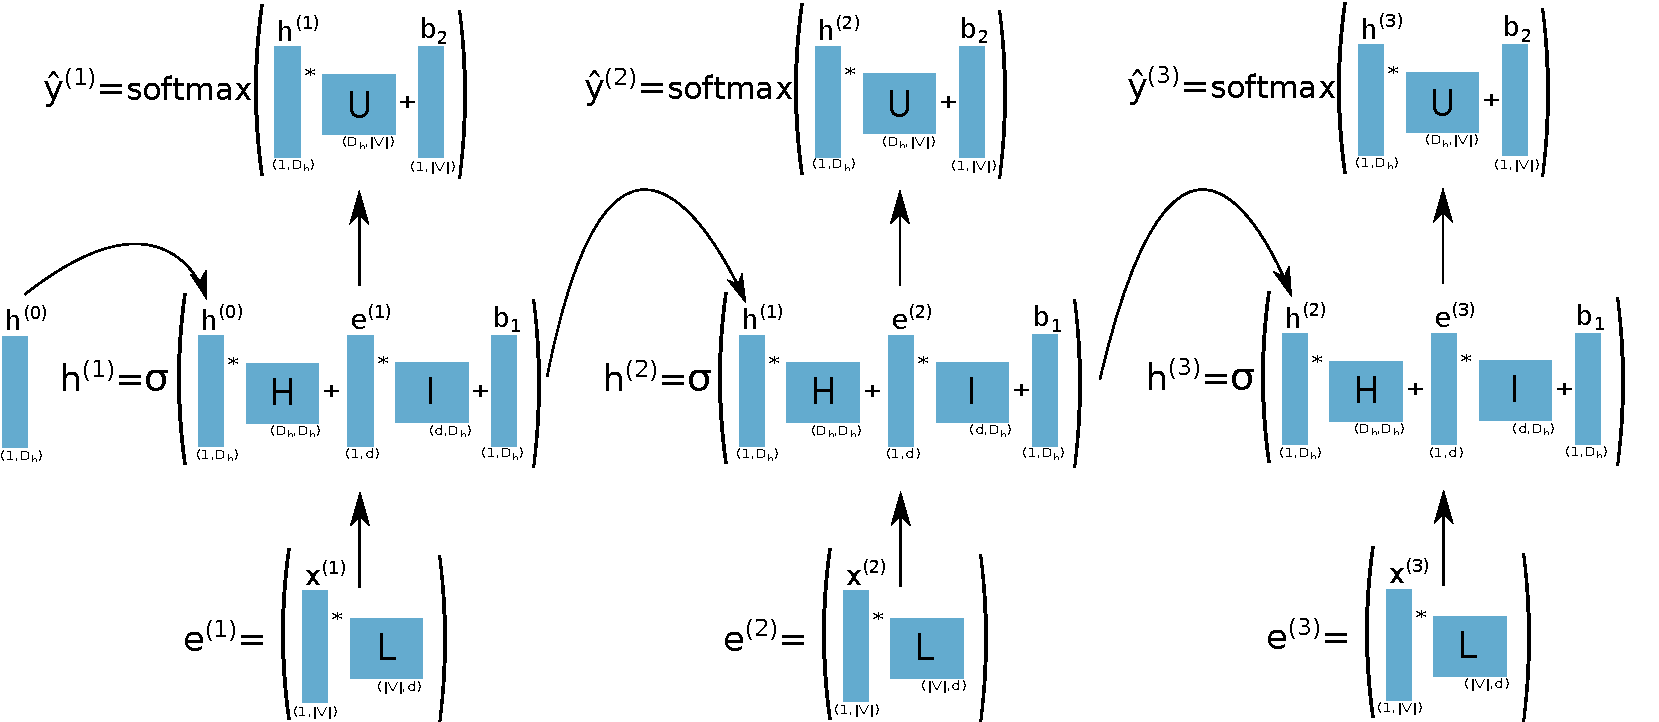
\includegraphics[scale=0.66]{RNN3.pdf}
\end{center}
\caption{A detailed representation of RNN for 3 time steps}
\label{RNN3}
\end{figure}
\textbf{This is a non-vectorized formulation.}\\
For $j \in \{1, \dots, d\}$:
\begin{equation}\label{eq:45}
\frac{\partial J^{(t)}}{\partial {L_{x^{(t-1)}}}}_{j} =\frac{\partial J^{(t)}}{\partial e^{(t-1)}_{j}} =\sum_{i=1}^{D_{h}}\frac{\partial J^{(t)}}{\partial h^{(t-1)}_{i}}\frac{\partial  h^{(t-1)}_{i}}{\partial  e^{(t-1)}_{j}}  = \sum_{i=1}^{D_{h}}\delta^{(t-1)}_{i}I_{i,j}
\end{equation}

For $i,j \in \{1, \dots, D_{h}\}$:


\begin{equation}\label{eq:46}
\frac{\partial J^{(t)}}{\partial H_{i,j}}\vert_{(t-1)} =\frac{\partial J^{(t)}}{\partial z^{(t)}_{j}}\frac{\partial  z^{(t)}_{j}}{\partial H_{i,j}}\vert_{(t-1)}  
\end{equation}
hence
\begin{equation}\label{eq:47}
\frac{\partial J^{(t)}}{\partial H_{i,j}}\vert_{(t-1)} =  \gamma^{(t,2)}_{j}(h^{(t-1)}_{i} + H_{j,j}\sigma^{\prime}(z^{(t-1)}_{j})h^{(t-2)}_{i})
\end{equation}



For $i \in \{1, \dots, d\}$ and $j \in \{1, \dots, D_{h}\}$:

\begin{equation}\label{eq:48}
\frac{\partial J^{(t)}}{\partial I_{i,j}}\vert_{(t-1)} =\frac{\partial J^{(t)}}{\partial z^{(t)}_{j}}\frac{\partial  z^{(t)}_{j}}{\partial I_{i,j}}\vert_{(t-1)}  
\end{equation}
thus
\begin{equation}\label{eq:49}
\frac{\partial J^{(t)}}{\partial I_{i,j}}\vert_{(t-1)} = \gamma^{(t,2)}_{j}(e^{(t)}_{i} + H_{j,j}\sigma^{\prime}(z^{(t-1)}_{j})e^{(t-1)}_{i})
\end{equation}

And for $j \in \{1, \dots, D_{h}\}$:

\begin{equation}\label{eq:50}
\frac{\partial J^{(t)}}{\partial {b_1}_{j}}\vert_{(t-1)} =\frac{\partial J^{(t)}}{\partial z^{(t)}_{j}}\frac{\partial  z^{(t)}_{j}}{\partial {b_1}_{j}}\vert_{(t-1)}  
\end{equation}
thus
\begin{equation}\label{eq:51}
\frac{\partial J^{(t)}}{\partial {b_1}_{j}}\vert_{(t-1)} = \gamma^{(t,2)}_{j}(1 + H_{j,j}\sigma^{\prime}(z^{(t-1)}_{j}))
\end{equation}

\textbf{3d)}
Give $h^{(t-1)}$, in one step of forward propagation we perform 4 matrix multiplication, 3 vector sums, one application of the sigmoid function in a vector of size $D_h$ and one application of the softmax function in a vector of size $|V|$. Let $f(D_h)$ and $g(|V|)$ be the cost of sigmoid function and the softmax function in that vectors, respectively. We can then express the cost with the equation:   

\begin{equation}\label{eq:52}
O(|V|d +D_hD_h + dD_h + 2D_h + f(D_h) +D_h|V| + |V| + g(|V|))
\end{equation}

Regarding backpropagation, assuming that $h^{(t-1)}$ if fixed, for each single step we perform 4 outer products, one Hadamard product, 2 matrix multiplication and one application of $\sigma^{\prime}$ in a vector of size $D_h$ (let $f^{*}(D_h)$ be the cost of this application). Let $\alpha$ be the following sum: 
\begin{equation}\label{eq:53}
\alpha = 2D_h|V| +D_h + f^{*}(D_h)+ 2dD_h + 2D_hD_h
\end{equation}
hence, for a backpropagation for a single step we have:
\begin{equation}\label{eq:54}
O(\alpha)
\end{equation}
and for $\tau$ steps
\begin{equation}\label{eq:55}
O(\tau\alpha)
\end{equation}

\textbf{3e)}

\begin{minted}{python}
def add_placeholders(self):
        # ## YOUR CODE HERE
        self.input_placeholder = tf.placeholder(tf.int32,
                                                shape=[None,
                                                       self.config.num_steps],
                                                name="input_placeholder")
        self.labels_placeholder = tf.placeholder(tf.int64,
                                                 shape=[None,
                                                        self.config.num_steps],
                                                 name="labels_placeholder")
        self.dropout_placeholder = tf.placeholder(tf.float32,
                                                  shape=[],
                                                  name="dropout_value")
        # ## END YOUR CODE
def add_embedding(self):
        with tf.device('/cpu:0'):
            # ## YOUR CODE HERE
            Lshape = (len(self.vocab), self.config.embed_size)
            L = tf.get_variable("L", shape=Lshape)
            look = tf.nn.embedding_lookup(L, self.input_placeholder)
            split = tf.split(1, self.config.num_steps, look)
            inputs = [tf.squeeze(tensor, squeeze_dims=[1]) for tensor in split]
            # ## END YOUR CODE
            return inputs    

def add_projection(self, rnn_outputs):
       
        # ## YOUR CODE HERE

        # shapes
        Ushape = (self.config.hidden_size, len(self.vocab))
        b2shape = (1, len(self.vocab))

        with tf.variable_scope("Projection_layer"):
            self.U = tf.get_variable("weights", shape=Ushape)
            self.b2 = tf.get_variable("bias", shape=b2shape)
            outputs = [tf.matmul(tensor, self.U) + self.b2
                       for tensor in rnn_outputs]

        # ## END YOUR CODE
        return outputs

def add_loss_op(self, output):
        # ## YOUR CODE HERE
        loss = sequence_loss([output],
                             [tf.reshape(self.labels_placeholder,
                              [self.config.batch_size * self.config.num_steps,
                               -1])],
                             [tf.constant(1.0)])
        # ## END YOUR CODE
        return loss

def add_training_op(self, loss):
        # ## YOUR CODE HERE
        optimizer = tf.train.AdamOptimizer(self.config.lr)
        train_op = optimizer.minimize(loss)
        # ## END YOUR CODE
        return train_op
        
def add_model(self, inputs):
        # ## YOUR CODE HERE

        rnn_outputs = []

        # shapes
        initialshape = (self.config.batch_size, self.config.hidden_size)
        Hshape = (self.config.hidden_size, self.config.hidden_size)
        Ishape = (self.config.embed_size, self.config.hidden_size)
        b1shape = (1, self.config.hidden_size)

        # initializers
        self.initial_state = tf.zeros(initialshape)

        with tf.variable_scope("RNN"):
            self.H = tf.get_variable("hidden_weights", shape=Hshape)
            self.I = tf.get_variable("input_weights", shape=Ishape)
            self.b1 = tf.get_variable("bias", shape=b1shape)

        previous_h = self.initial_state

        for i, tensor in enumerate(inputs):
            with tf.variable_scope("RNN", reuse=True):
                drop_tensor = tf.nn.dropout(tensor, self.config.dropout)
                h = tf.sigmoid(tf.matmul(previous_h, self.H) +
                               (tf.matmul(drop_tensor, self.I) + self.b1))
                h = tf.nn.dropout(h, self.config.dropout)
                rnn_outputs.append(h)
                previous_h = h
                if i == (len(inputs)-1):
                    self.final_state = h
        # ## END YOUR CODE
        return rnn_outputs
\end{minted}

After some experiments we choose the following hyper parameters: $ batch\_size=104, dropout=0.991323729933, lr=0.00217346380124, num\_steps=14$. This choice yields validation perplexity = $163.170974731$. As can be seen in the plots from Figure \ref{RNN_e} we could continue searching better hyper parameters, but due the lack of time (we use CPU only) we decide to stop the search at those parameters.

\begin{figure}[H] 
  \begin{subfigure}[b]{0.5\linewidth}
    \centering
    \includegraphics[width=1.05\linewidth]{RNNLM_batch_pp.png} 
    \caption{Perplexity vs batch size} 
    \label{rnn_batch} 
    \vspace{4ex}
  \end{subfigure}%% 
  \begin{subfigure}[b]{0.5\linewidth}
    \centering
    \includegraphics[width=1.05\linewidth]{RNNLM_dropout.png} 
    \caption{Perplexity vs dropout} 
    \label{rnn_dropout} 
    \vspace{4ex}
  \end{subfigure} 
  \begin{subfigure}[b]{0.5\linewidth}
    \centering
    \includegraphics[width=1.05\linewidth]{RNNLM_lr.png} 
    \caption{Perplexity vs learning rate} 
    \label{rnn_lr} 
  \end{subfigure}%%
  \begin{subfigure}[b]{0.5\linewidth}
    \centering
    \includegraphics[width=1.05\linewidth]{RNNLM_step_pp.png} 
    \caption{Perplexity vs step size} 
    \label{rnn_step} 
  \end{subfigure} 
  \caption{Experiments with the RNN language model}
  \label{RNN_e} 
\end{figure}

\textbf{3f)}

\begin{minted}{python}
def generate_text(session, model, config, starting_text='<eos>',
                  stop_length=100, stop_tokens=None, temp=1.0):
    state = model.initial_state.eval()
    tokens = [model.vocab.encode(word) for word in starting_text.split()]
    for i in xrange(stop_length):
        # ## YOUR CODE HERE
        feed = {model.input_placeholder: [[tokens[-1]]],
                model.initial_state: state,
                model.dropout_placeholder: 1.0}
        state, y_pred = session.run([model.final_state, model.predictions[-1]],
                                    feed_dict=feed)
        # ## END YOUR CODE
\end{minted}
Examples of generated sentence:

\begin{itemize}
\item \textbf{$>$ sex is:} sex is chairman of two-year operation $<$eos$>$

\item \textbf{$>$ violence is:} violence is expected well but by the german social concept of public conditions around what if the sec $<$unk$>$ with fujis at greenville odd a $<$unk$>$ formerly won away with editor of the federal court term the news spokeswoman says mr. $<$unk$>$ said the $<$unk$>$ 's is one location of the development of a new active position he says dick green louisville ky. representatives of l.j. hooker maker increased N N to N at N $<$eos$>$

\item \textbf{$>$ this is a great:} this is a great japanese she had the president maker was the ceo for a time when i do n't any shared with potential but going to be hampered by the noriega is that last winter $<$eos$>$
\end{itemize}

\end{document}
